%!TEX root = ../scivis_lbaakman_bvanloon.tex

\begin{figure}
	\centering
	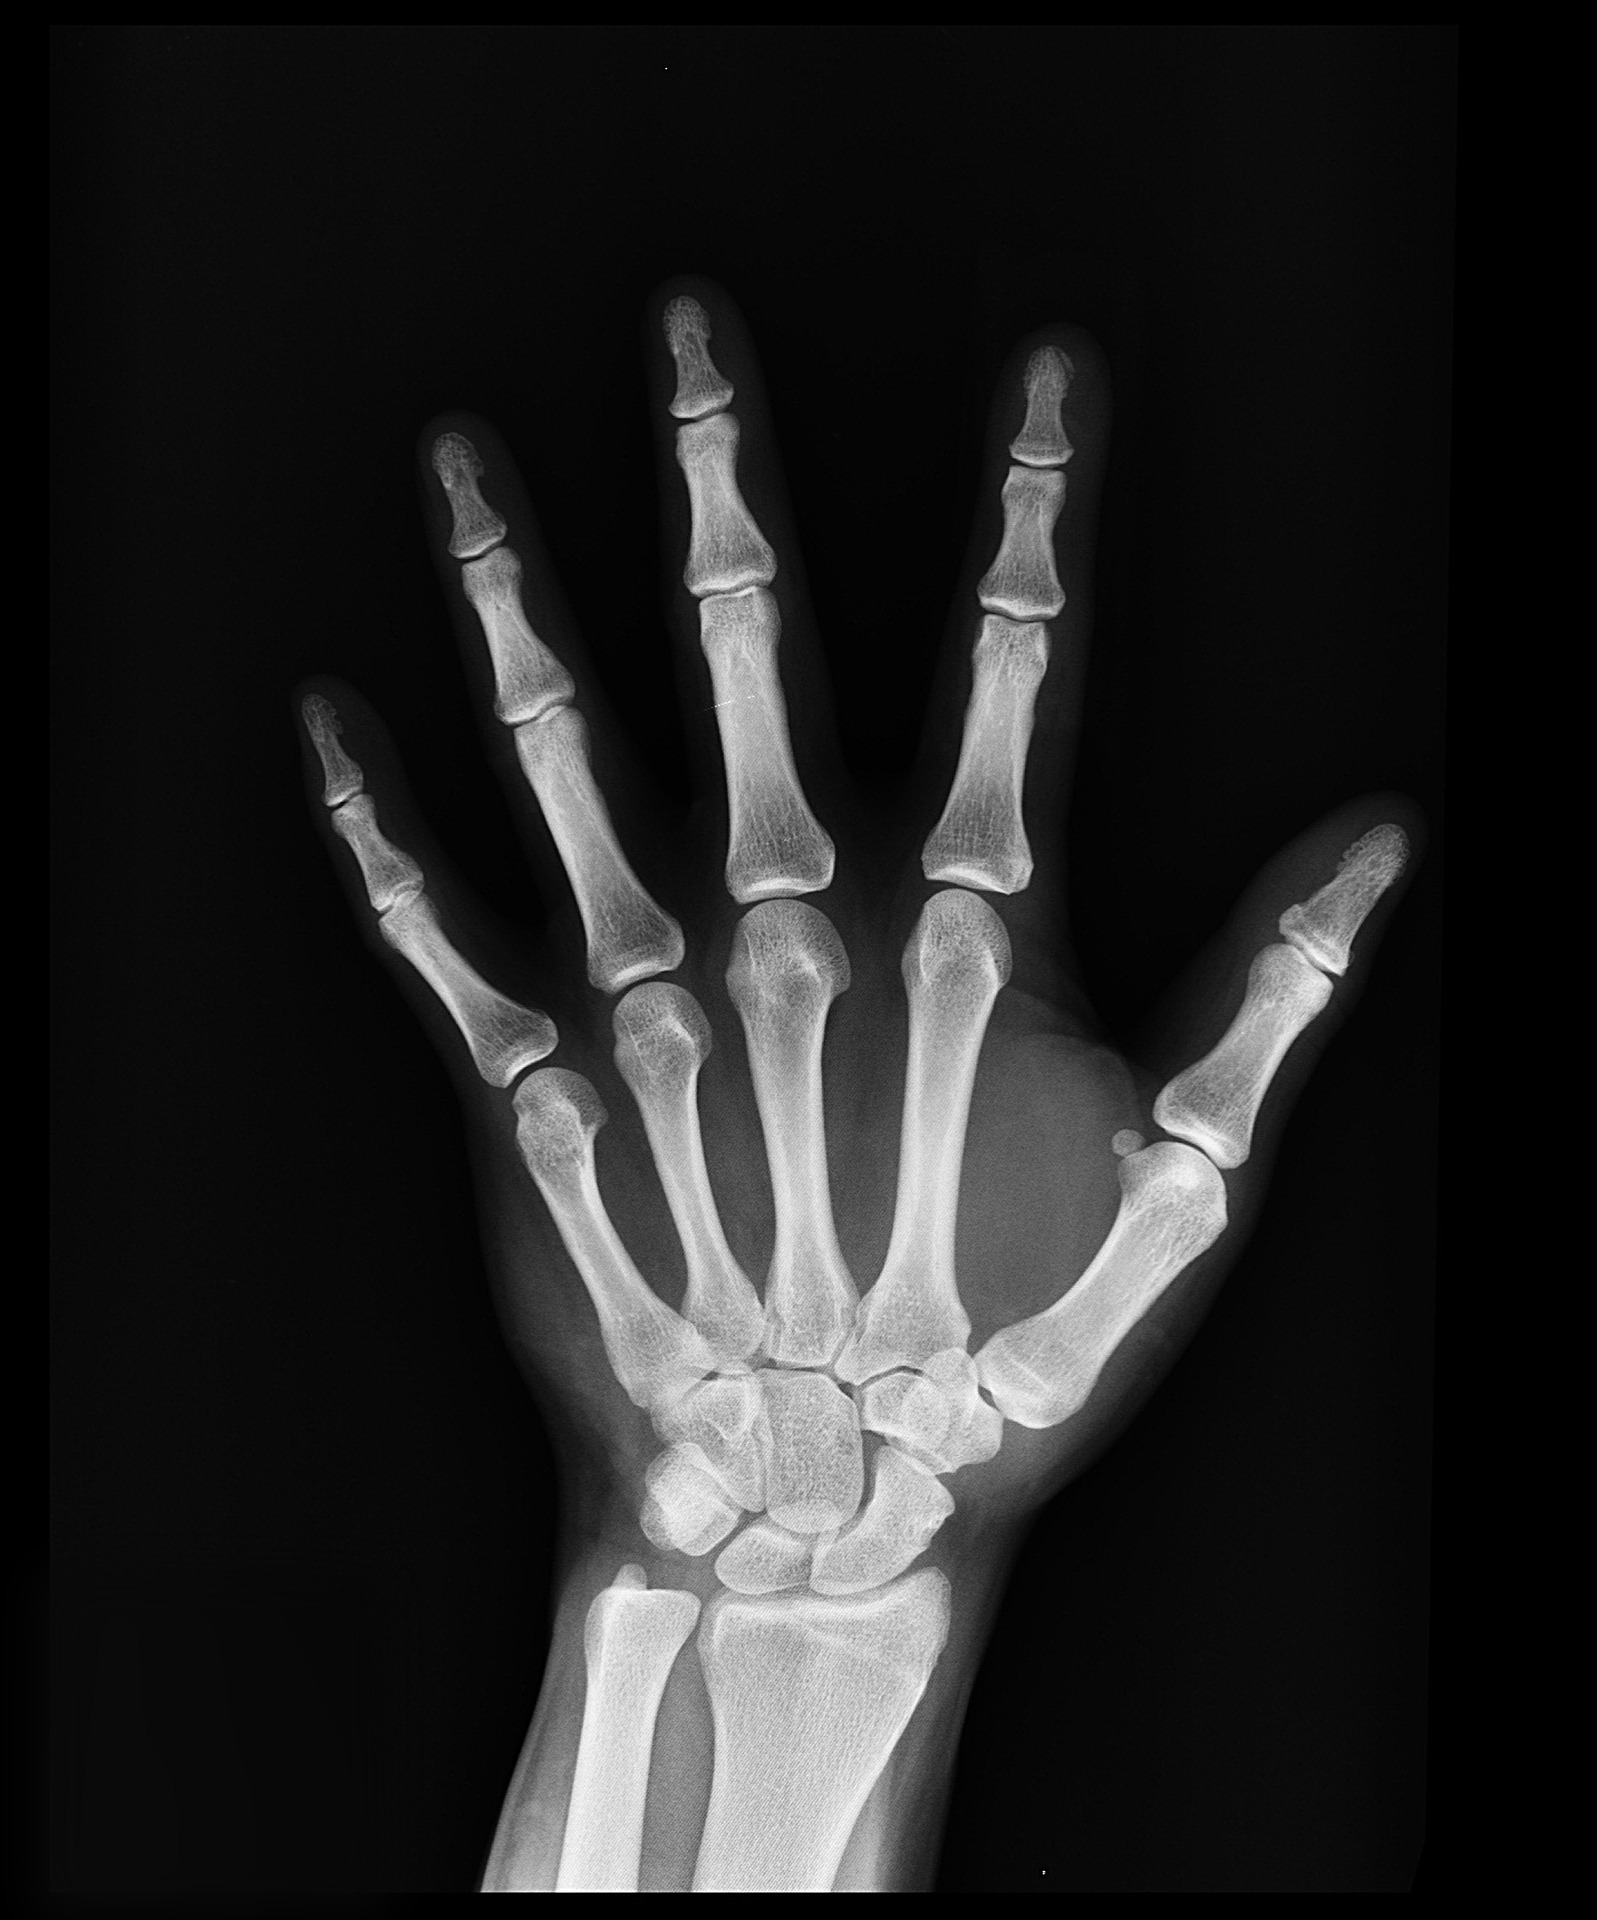
\includegraphics[width=0.5\textwidth, height=0.2\textheight, keepaspectratio]{colormapping/img/x-ray.jpg}
	\caption{An example of the use of a color map, image from \cite{xray}.}
	\label{fig:colormapping:xray}
\end{figure}

\Cref{fig:colormapping:xray} shows a well known example of the use of a color map. In this image lighter colors are used to indicate areas where the density of the X-rayed object are high, whereas darker colors represent areas of low density. X-rays use gray scale color maps, that is it maps the density values of the object to colors ranging from black to white. \Cref{s:colormapping:introduction} discusses the gray scale color map extensively and introduces other color maps. In \cref{ss:colormaps:parameterization} the parameterization of these color maps is introduced. \Cref{ss:colormaps:applying} discusses techniques that can be used to map the scalar data to the color maps. In the final section, \cref{ss:colormaps:variables}, the application of the color maps to the scalar variables in our application is discussed. 

\subsection{Different Color Maps}
\label{ss:colormaps:differentmaps}

\begin{figure}
	\centering
	\begin{subfigure}{\textwidth}
		\centering
		\includegraphics[width=\textwidth]{./img/_}
		\caption{Rainbow color map, $\varDX = 0.8$.}
		\label{fig:colormapping:intro:differntColorMaps:rainbow}
	\end{subfigure}
	\begin{subfigure}{\textwidth}
		\centering
		\missingfigure{ColorMap to be generated}
		% \includegraphics[width=\textwidth]{./img/_}
		\caption{Gray scale color map.}
		\label{fig:colormapping:intro:differntColorMaps:grayscale}
	\end{subfigure}	
	\begin{subfigure}{\textwidth}
		\centering
		% \includegraphics[width=\textwidth]{./img/_}
		\missingfigure{ColorMap to be determined}
		\caption{Undetermined color map.}
		\label{fig:colormapping:intro:differntColorMaps:ofChoice}
	\end{subfigure}		
	\caption{A visualization of different color maps: \subref{fig:colormapping:intro:differntColorMaps:rainbow} rainbow, \subref{fig:colormapping:intro:differntColorMaps:grayscale} gray scale, and \subref{fig:colormapping:intro:differntColorMaps:ofChoice} unknown color map.}
	\label{fig:colormapping:introduction}
\end{figure}

	% Rainbow ColorMap
	\todo[inline]{Discuss Rainbow colormap: advantages, disadvantages, influence of dx}		

	% GrayScale ColorMap
	\todo[inline]{Discuss GrayScale color map: advantages, disadvantages}

	% ColorMap of Choice
	\todo[inline]{Discuss Chosen color map: advantages, disadvantages, why this one}
	

	

\subsection{Parameterization of Color Maps}
\label{ss:colormaps:parameterization}
	\todo[inline]{Number of colors, disadvantages/advantages when to use?}
	\todo[inline]{Change hue, disadvantages/advantages when to use?}
	\todo[inline]{Change saturation, disadvantages/advantages when to use?}

\subsection{Applying Color Maps}
\label{ss:colormaps:applying}
	\todo[inline]{Discuss clamping}
	\todo[inline]{Discuss scaling}

\subsection{Variables that the Color Maps are Applied to}
\label{ss:colormaps:variables}
	\todo[inline]{Discuss fluid density, what is it? suitable for colormapping? Which colormap?}
	\todo[inline]{Discuss fluid velocity magnitude what is it? suitable for colormapping? Which colormap?}
	\todo[inline]{Discuss force field magnitude what is it? suitable for colormapping? Which colormap?}
